\chapter{Additional Qualitative Results}\label{app:qualitative}
\section{Selection and interpretation}
The qualitative recorder uses the same working resolution, feature budget, matching seed and verification policy as the comparison. For each documented protocol, it prefers a positive pair accepted by the learned method but rejected by SIFT; if none exists, a fixed final-pair fallback is used. Coordinates, masks and transforms are saved in \code{results/qualitative_matches.json}. These figures are illustrative selections, not an unbiased sample of overall performance.

\begin{figure}[htbp]\centering
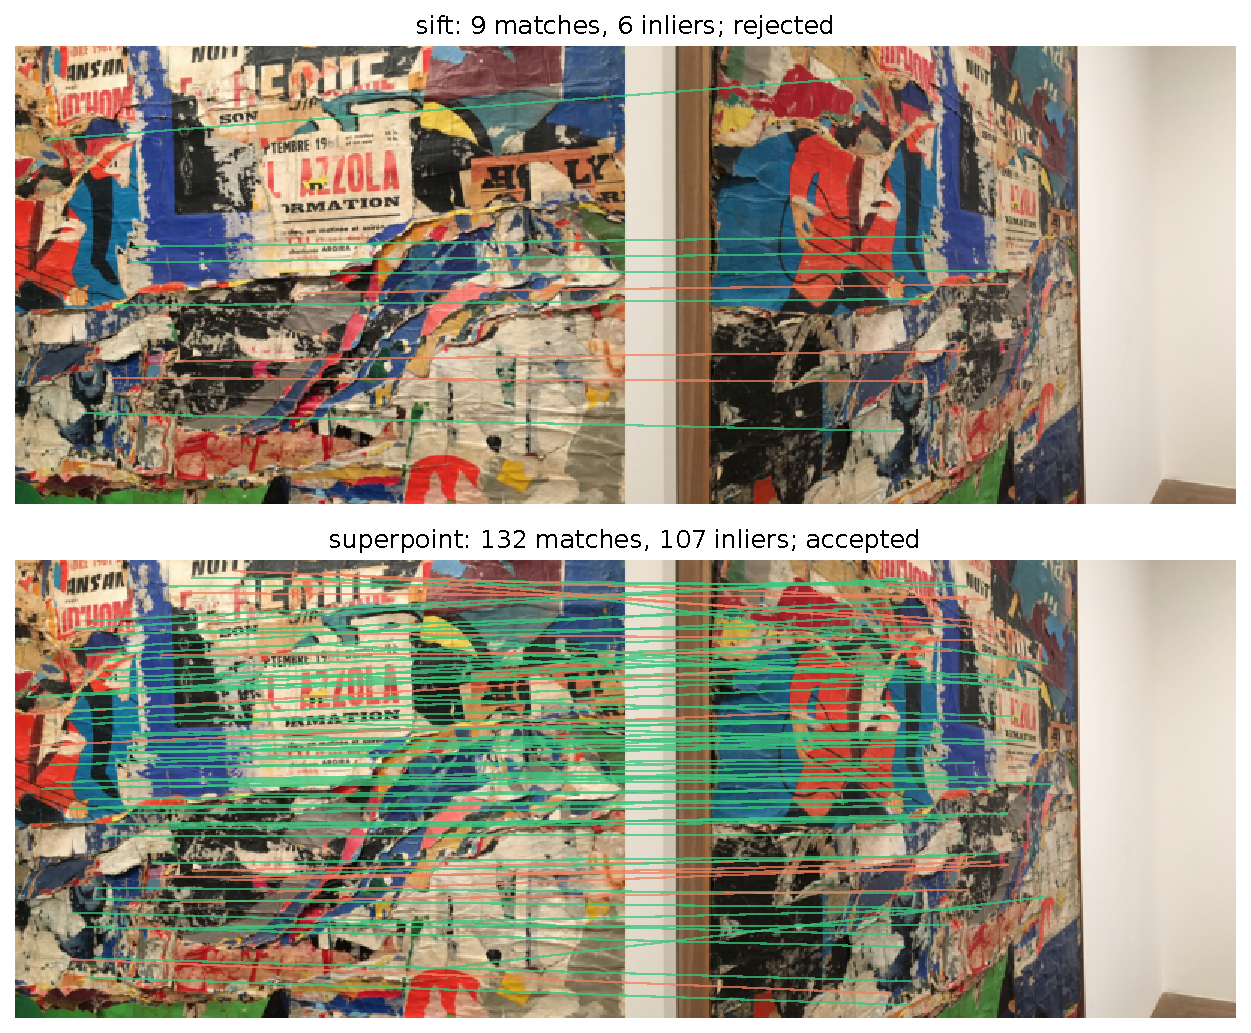
\includegraphics[width=\textwidth,height=.78\textheight,keepaspectratio]{matches_hpatches_viewpoint.pdf}
\caption{Actual matching on the selected HPatches viewpoint example. Sparse visual support and boundary extrapolation should be considered alongside the aggregate corner-error results.}\label{fig:matches-viewpoint}
\end{figure}
\Cref{fig:matches-viewpoint} complements the illumination example in the main chapter. RANSAC inlier status means compatibility with the fitted homography, not a manually established physical correspondence label. Up to eighty lines are displayed to preserve readability; full point arrays remain in the recorded artifact.

\begin{figure}[htbp]\centering
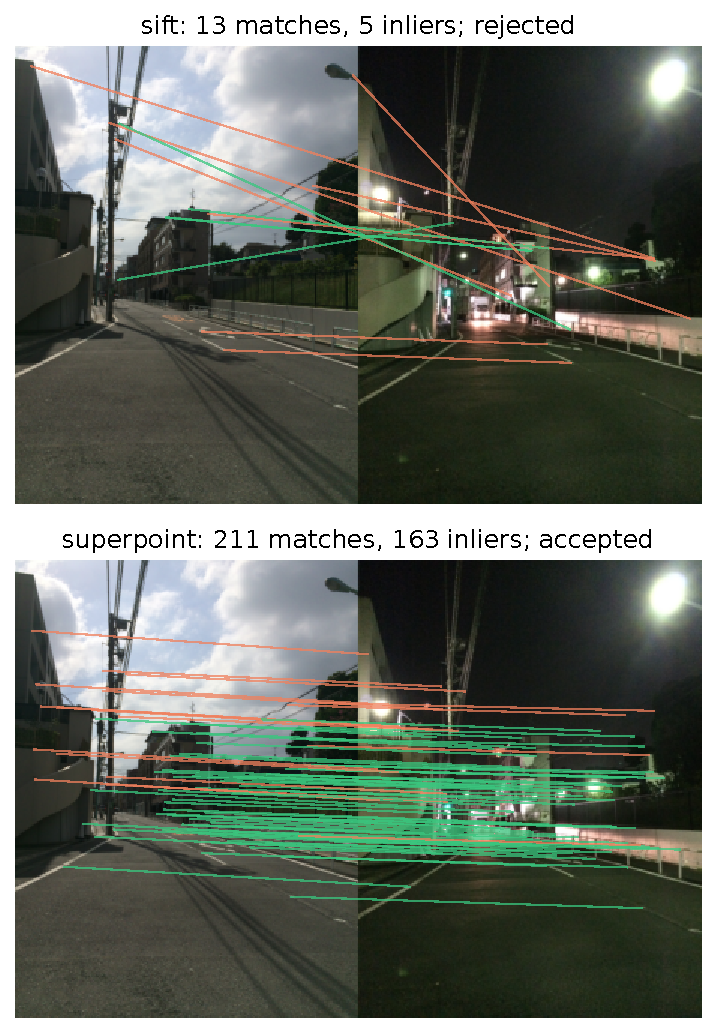
\includegraphics[width=\textwidth,height=.78\textheight,keepaspectratio]{matches_tokyo_day_to_night.pdf}
\caption{Executed local correspondences across a real selected Tokyo day/night pair. The fitted map is not evaluated as a metric pose or ground-truth planar alignment.}\label{fig:matches-night}
\end{figure}
\Cref{fig:matches-night} shows that actual cross-time photographs, rather than only generated darkness, contribute to the comparison. The selection supports a visual explanation of the measured local-support difference. It cannot establish that all visible depths share one plane or that the resulting overlay is a calibrated world-space object.

\begin{figure}[htbp]\centering
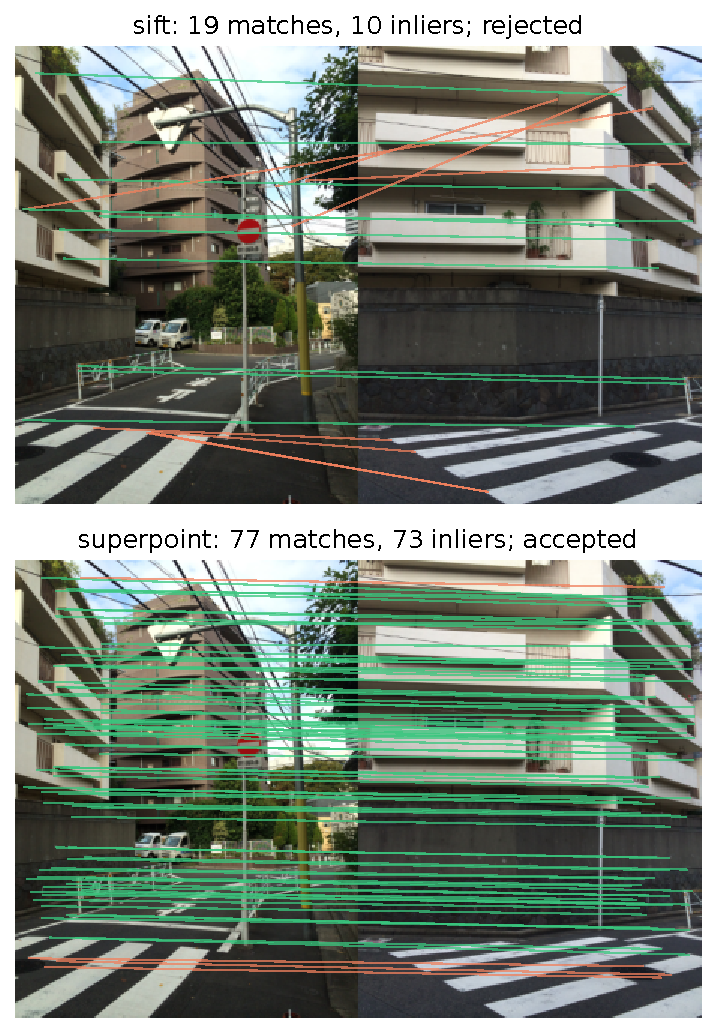
\includegraphics[width=\textwidth,height=.78\textheight,keepaspectratio]{matches_tokyo_day_to_day.pdf}
\caption{Actual matching for the selected daytime direction-change pair. This protocol tests reduced scene overlap despite unchanged daylight labels.}\label{fig:matches-day}
\end{figure}
\Cref{fig:matches-day} illustrates why daylight alone does not guarantee a useful anchor. The complete ranked predictions and accepted/rejected decisions, including wrong-place acceptances, are available for every query. Readers should inspect those aggregate records before drawing a method ranking from one figure.

\section{Demo provenance}
The comparison video is generated from the documented selected real daytime and night photographs, with small known two-dimensional motion applied to form query clips. This is explicitly labelled in the frames. The demo executes classical and full recognition independently on those queries and stores frame-level decisions and measured latency. No ground-truth homography is substituted when a recogniser fails.

The animation is a downsampled presentation of the same recorded rendered frames. Its playback rate is chosen for viewing and does not represent inference speed. The source-video regression and CLI video output remain separate artifacts, because real temporal input and motion synthesised from still images provide different evidence.
